\documentclass[12pt,fleqn]{report} %taille de la police par défaut, et équations jusitifées à gauche
\usepackage[top=3cm,bottom=3cm,left=3.2cm,right=3.2cm,headsep=10pt,a4paper]{geometry}
\usepackage{xcolor}
\definecolor{enstabGreen}{HTML}{C8D200} 	%vert  	#c8d200 
\definecolor{enstabLightGreen}{HTML}{E9ED99} 	%vert  	#c8d200 
\definecolor{enstabLightBlue}{HTML}{009EE0} %bleu clair 	#009ee0
\definecolor{enstabVeryLightBlue}{HTML}{99D8F3} %bleu clair 	#009ee0
\definecolor{enstabDarkBlue}{HTML}{005C8F}	%bleu foncé 	#005c8f
\definecolor{enstabDarkGrey}{HTML}{333333}	%gris fort 	#333333
\definecolor{enstabLightGrey}{RGB}{48,48,48}	%gris fort 	#333333
\definecolor{enstabParme}{HTML}{8878B2}		%parme 	#8878b2
\definecolor{enstabOrange}{HTML}{F18E00} 	%orange 	#f18e00
\usepackage[colorlinks=true,
        urlcolor=enstabLightBlue,
        anchorcolor=enstabDarkBlue,
        linkcolor=enstabDarkBlue,
        citecolor=enstabDarkGrey,
        pdfauthor={O. Reynet},
        pdfkeywords={LaTeX; Report},
        pdftitle={How to produce a report with LaTeX},
        pdfsubject={yours !}] {hyperref}
\usepackage{url}
\usepackage[utf8]{inputenc} % lettres accentuées
\usepackage[T1]{fontenc}    % Use 8-bit encoding that has 256 glyphs
\usepackage[frenchb]{babel} % Pour le français
\usepackage{eso-pic}        % pour une image en fond, page de titre
\usepackage{graphicx}       % Pour inclure des images
\graphicspath{{images/}}    % Où sont les images ?

\usepackage{listings}      % Pour coloriser les codes que vous insérez
\lstset{ %
  backgroundcolor=\color{white},   % choose the background color; you must add \usepackage{color} or 
  basicstyle=\footnotesize\ttfamily,        % the size of the fonts that are used for the code
  breakatwhitespace=false,         % sets if automatic breaks should only happen at whitespace
  breaklines=true,                 % sets automatic line breaking
  captionpos=b,                    % sets the caption-position to bottom
  commentstyle=\color{enstabOrange},    % comment style
  deletekeywords={...},            % if you want to delete keywords from the given language
  escapeinside={\%*}{*)},          % if you want to add LaTeX within your code
  extendedchars=true,              % lets you use non-ASCII characters; for 8-bits encodings only, does not work with UTF-8
  %frame=single,                    % adds a frame around the code
  keepspaces=true,                 % keeps spaces in text, useful for keeping indentation of code (possibly needs columns=flexible)
  keywordstyle=\color{enstabDarkBlue},       % keyword style
  %language=Octave,                 % the language of the code
  morekeywords={*,...},            % if you want to add more keywords to the set
  numbers=left,                    % where to put the line-numbers; possible values are (none, left, right)
  numbersep=8pt,                   % how far the line-numbers are from the code
  numberstyle=\tiny\color{enstabDarkGrey}, % the style that is used for the line-numbers
  rulecolor=\color{black},         % if not set, the frame-color may be changed on line-breaks within not-black text (e.g. comments (green here))
  showspaces=false,                % show spaces everywhere adding particular underscores; it overrides 'showstringspaces'
  showstringspaces=false,          % underline spaces within strings only
  showtabs=false,                  % show tabs within strings adding particular underscores
  stepnumber=5,                    % the step between two line-numbers. If it's 1, each line will be numbered
  stringstyle=\color{enstabParme},     % string literal style
  tabsize=2,                       % sets default tabsize to 2 spaces
  title=\lstname                   % show the filename of files included with \lstinputlisting; also try caption instead of title
}





\usepackage{booktabs}       % pour de jolis tableaux
%\usepackage{fancyhdr}       % pour des entêtes et pieds de pages améliorés.
\usepackage{makeidx}        % requis pour faire les index
\usepackage{amsmath}
\usepackage{amsfonts}
\usepackage{amssymb}
\usepackage{color}
\usepackage{array}
\usepackage{graphicx}
\usepackage{caption} 
\usepackage{hyperref}
\usepackage{algorithm}
\usepackage{algorithmic}
\usepackage{times}
\usepackage{tabularx}     % Ce fichier contient tous les packages nécessaires à la compilation

\begin{document}
\renewcommand{\contentsname}{Contents}	% Nom pour la table des matières
\renewcommand{\bibname}{Bibliography}	% Nom pour les références bibliographiquessss


%----------------------------------------------------------------------------------------
%	PAGE DE GARDE
%----------------------------------------------------------------------------------------

\begingroup
\thispagestyle{empty}
\AddToShipoutPicture*{\put(6,5){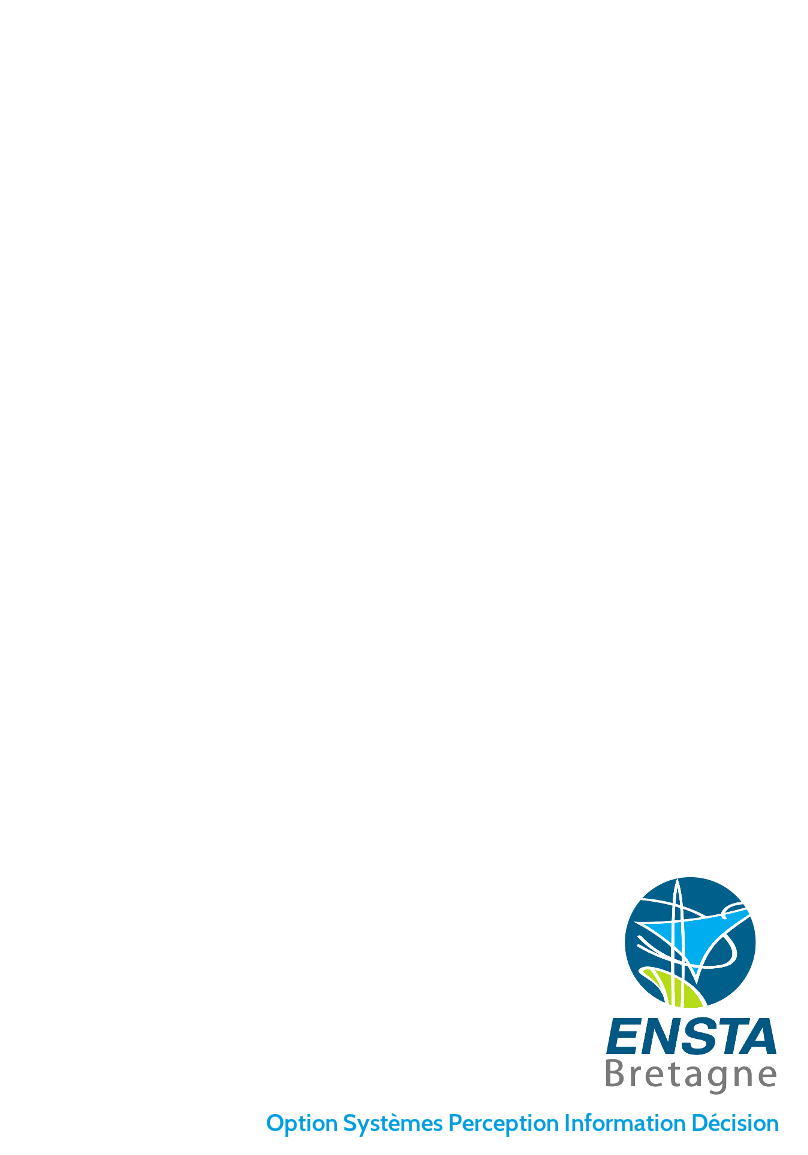
\includegraphics[scale=1]{FondTitreSPID}}} % Image background
\begin{center}
\vspace*{2cm}
{\Huge \textsc{\textbf{Report}}}\\


\vspace*{2cm}
{\huge Surveillance Of The Bay Of Biscay}\par % Intitulé du projet
\end{center}


\vspace*{4cm}
\textbf{\LARGE rédigé par :} 
\begin{center}
{\LARGE
\begin{tabular}{cc}
Elouan Autret & Thomas Boulier\\
Maxime Bouyssou & Philippe Chuzel\\
Alice Danckaers & David Duverger\\
Raphael Finkelstein & Sylvain Hunault\\
Pierre Jacquot & Mael Le Gallic\\
Eric Mourre & Thiago Oliveira\\
Benoit Raymond & Khadimoullah Vencatasamy\\
\end{tabular}}
\end{center}


\vspace*{1.5 cm}
{\LARGE \textbf{sous la direction de :}}\\
\begin{center}
{\LARGE
Luc Jaulin\\
Benoit Zerr\\}
\end{center}
\endgroup



%----------------------------------------------------------------------------------------
%	SOMMAIRE
%----------------------------------------------------------------------------------------
\tableofcontents  % Imprime le sommaire
\cleardoublepage  % pour commencer sur une page impaire


%----------------------------------------------------------------------------------------
%	Préambules
%----------------------------------------------------------------------------------------
\chapter*{Acknowledgement}
\addcontentsline{toc}{chapter}{Acknowledgement}

\chapter{Remerciements}
\epigraph{La gratitude est non seulement la plus grande des vertus, mais c'est également la mère de tous les autres.}{Emil Cioran}




%----------------------------------------------------------------------------------------
%	PART I 
%----------------------------------------------------------------------------------------
\chapter{Introduction}
\bigskip

The goal of this project is to ensure the security of the Bay of Biscay by detecting any intruder entering this maritime area.
A group of robots, equipped with GPS, are being used thanks to specific algorythms and a particular monitoring strategy.

\bigskip

In order to proceed with the project, the following working hypotheses are considered:
\begin{itemize}
\item The simulation can be done in a two-dimensional world ;
\item Intruders will have a constant given velocity throughout the simulation ;
\item Every surveillance robot has a detection range of $d_{i}$ within which an itruder is necessarily detected ;
\item The safe zones are as a group of rectangles where the intruder can not be.
\end{itemize}

\bigskip

Two deliverables will be delivered:
\begin{itemize}
\item The first one is a theoretical simulation written to a large extent in Python 3.0 which will allow to determine whether or not the used algorythms are relevant ;
\item The second one is a practical simulation using some buggies robots available in the robotics group of ENSTA Bretagne.
\end{itemize}




%----------------------------------------------------------------------------------------
%	PART II 
%----------------------------------------------------------------------------------------
\chapter{Secure zone processing}

\section{Introduction to interval analysis}

\documentclass[a4paper,12pt]{report}
 
\usepackage[latin1]{inputenc}
\usepackage{graphicx}

\begin{document}
    \section{Interval Analysis}
    
	\vspace{0.5 cm}
	
	 For this project, we have chosen the intervals calculation    approach which guarantees solutions in a given interval of uncertainty.

	\vspace{0.5 cm}
	
	In the Intervals theory, a known value is replaced by an interval with a certain uncertainty in which it is sure that this measure is include. So, for a known value x, the corresponding interval is $\ [x-\epsilon, x+\epsilon] $.


    \begin{center} 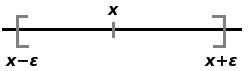
\includegraphics[scale=0.8]{Interval.png} \end{center}
    
    The goal of this method is to give the percentage of certainty which allows to obtain reliable and robust results. In tow dimensions, intervals are represented by boxes. Here is an example of the resolution by Intervals. It is the result of S1|S2 with:
    
    	\vspace{0.6 cm}
    	

    \begin{center} 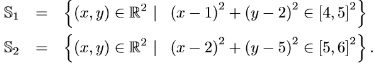
\includegraphics{Formule1.png} \end{center}
    
    \begin{figure}[!h] 
    \center
    	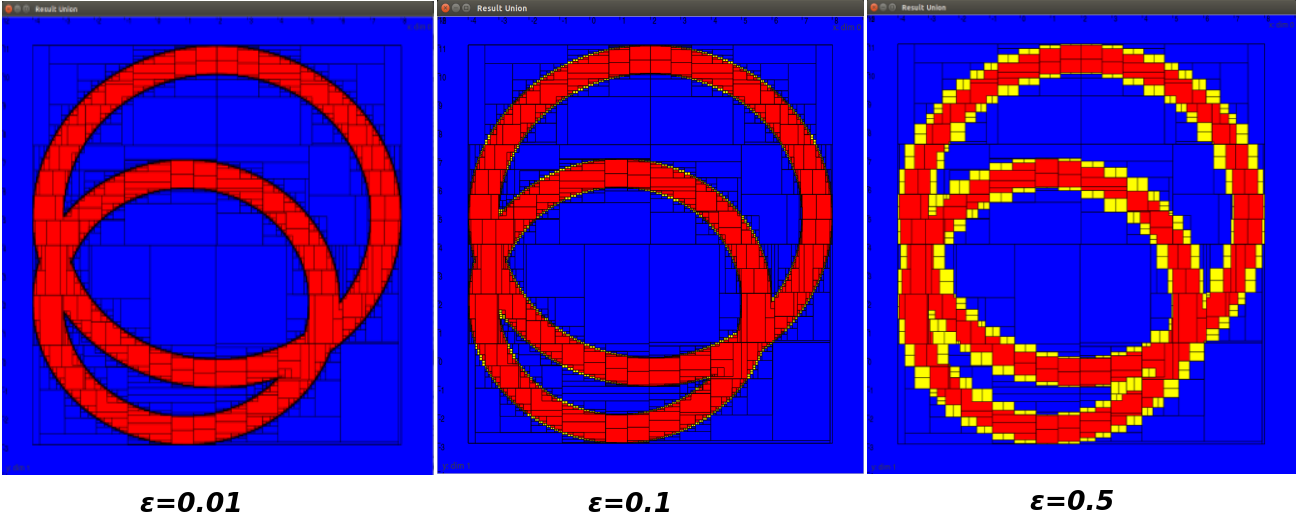
\includegraphics[scale=0.4]{Boxes.png} 
    	\caption{Resolution of S1 U S2 for different precision with intervals calculation } 
    \label{S1 U S2}
	\end{figure} 

	\newpage

	If a box frames a solution, it is cut in two parts and the calculation is reiterated on these two boxes which allow to discriminate one of them and to reduce solutions. However, this operation take lot of time because the number of boxes increase of  2n each time. That is why, the contractors are used, they allow to refine the boxes at the intervals which include strictly the solution before to cut them. This method allow to have an important gain of time during the simulation. 

	\begin{figure}[!h] 
    \center
    	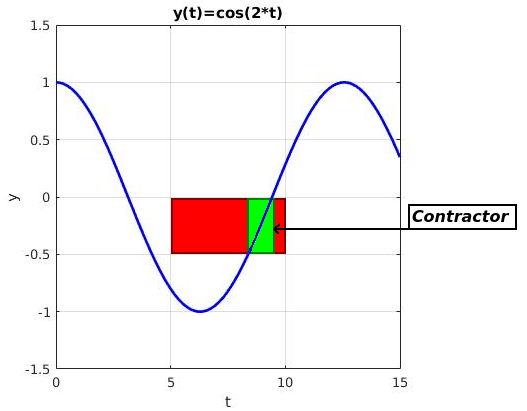
\includegraphics[scale=0.8]{Contractor.png} 
    	\caption{Example of the utilisation of contractor} 
    \label{Contractor}
	\end{figure} 
	
	For the example, the signal cos(2*t) in blue is used. The box in red corresponds to the normal box and the green box corresponds to the contractor. With this example, we can easily see that contractors improve  the simulation in terms of time. 

	\vspace{0.5 cm}
	
	For the simulation of the Gascogne project, we used a SIVIA function which make the paving for the representation of the France, robots control and their erosion.
	
	
\end{document}



\section{Secure zone estimation with interval analysis}
\vspace{0.5 cm}
\textcolor{blue} {\textit{Elouan AUTRET}}
\vspace{0.3 cm}
\subsection{Thick Functions}

A thick function is a function of $\mathbb{R^{\textnormal{\ensuremath{n}}}}$ in $\mathbb{R^{\textnormal{\ensuremath{p}}}}$ that associate to an element x $\in \mathbb{R^{\textnormal{\ensuremath{n}}}}$ a convex element of $\mathbb{R^{\textnormal{\ensuremath{p}}}}$ where there can have intervals as parameters of the function.

For example, consider the function f :
\begin{algorithmic}[H]
\STATE f :  $\mathbb{R} \rightarrow \mathbb{R} $
\STATE $\mathbf{x} \rightarrow \mathbf{x}+ \mathbb{[ \,\textnormal{1},\textnormal{2}] \,}$
\end{algorithmic}

If the width of x is null (ex: [1,1]) the width of f(x) will be strictly greater than zero ([2,3]) (see figure~\ref{fig:thickFunction}).

A thick function can be consider as an interval of classical function with the same principal properties like an lower bound and an upper bound, [f] is equal to [$f^{\textnormal{\ensuremath{-}}}$,$f^{\textnormal{\ensuremath{+}}}$]  where $f^{\textnormal{\ensuremath{-}}}$ is the lower bound function and $f^{\textnormal{\ensuremath{+}}}$ is the upper one. See the example for  a function from $\mathbb{R} $ in$ \mathbb{R} $ :

\begin{figure}[H]
\centering
    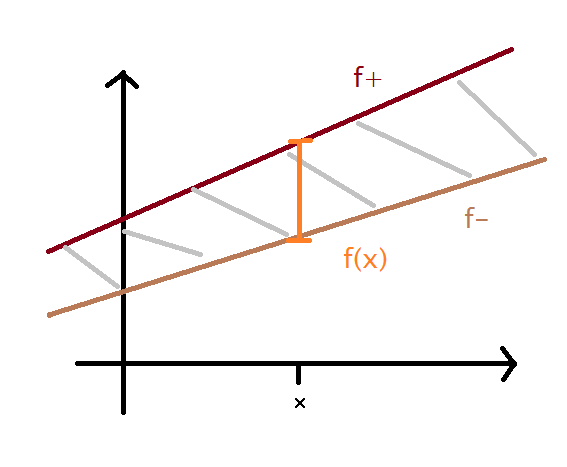
\includegraphics[scale=0.8,angle=0]{thick_function.png}
    \caption{Example of a thick function  $\mathbb{R} \rightarrow \mathbb{R} $.}
    \label{fig:thickFunction}
\end{figure}

Those thick functions allow, for the surveillance problem, the modelling of the uncertainty of
the position of the boat that will watch the bay.\\
Indeed, the position can be given by a GPS but the result is not absolute, the real position can be off by a few meters, for example if [1,2] is the position of the boat and 10 is the range of detection by the boat, then the set of the secure zone without uncertainty would be:

\begin{equation}
 \mathbf{S} = \{ x \in \mathbf{R}^{\textnormal{\ensuremath{2}}} | (x(1)-1)^{\textnormal{\ensuremath{2}}} + (x(2)-2)^{\textnormal{\ensuremath{2}}} \leq 100 \}  \label{eqDIST}
\end{equation}

But if we add an uncertainty of 0.5 to the position then the set become:
\begin{equation}
 \mathbf{S} = \{ x \in \mathbf{R}^{\textnormal{\ensuremath{2}}} | (x(1)-[ \,0.5,1.5] \,)^{\textnormal{\ensuremath{2}}} + (x(2)-[ \,1.5,2.5] \,)^{\textnormal{\ensuremath{2}}} \leq 100 \}  \label{eqDISTTHICK}
 \end{equation}

This set can easily be found with interval analysis using the ibex library with a separator for the precedent equation ~\eqref{eqDIST}, then by proceeding with the SILVIA algorithm and associating the code with VIBES (a viewer tool) the zones reached by the boat can be visualized:

\begin{figure}[H]
\centering
    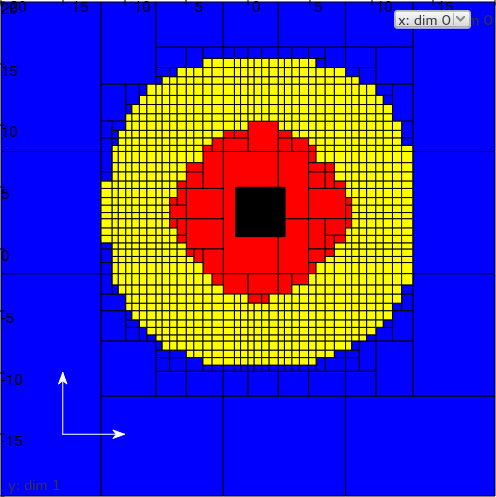
\includegraphics[scale=0.8,angle=0]{1_boat_no_efficient_border.png}
    \caption{Zone secured by one boat in red, yellow zone is uncertain,blue is not secured,the black square are the possible position of the boat.}
    \label{fig:SecureZoneOneBoat}
\end{figure}

The figure~\ref{fig:SecureZoneOneBoat} shows the zone covered by the surveillance boat, in red the zone is certain to be covered, in yellow it is not sure it depends on the real place of the boat in the black square or uncertainty.

\subsection{Test for Biscay Bay Surveillance}
For all this section we consider that for all $\mathbf{X} \in \mathbb{R^{\textnormal{\ensuremath{2}}}}$,  $\mathbf{X}$ is included in the bay of Biscay (the set $\mathbb{G}$) in order to facilitate the comprehension.\\
The figure~\ref{fig:SecureZoneOneBoat} shows that the zone covered by the boats can be found but it also point out that the computing of the zone is not efficient, the uncertain zone cannot be classifyasout or in the secured zone so the SIVIA algorithm cut the boxes to their minimal size even if it is possible to know their status of uncertainty thus proceeding to more computation than needed, a new test is required instead of a simple separator to allow a faster and cleaner computation of the secured zone.
The test can be found in the algorithm ~\ref{alg:one_boat_alg} which take a box (an element of $\mathbb{R}^{\textnormal{\ensuremath{2}}}$)) and determine its status, the state can vary between six status where for now the border regroup more or less three status as it can be seen in the following table:

\begin{center}
\begin{tabular}{|m{0.10\linewidth}|m{0.15\linewidth}|m{0.5\linewidth}|}
\hline
 Symbol & In Algorithm  & Meaning  \\ \hline
 0 & OUT & Box is not in the Secure Zone  \\ \hline
 1 & IN & Box is in the secure zone \\ \hline
 ? & UNKNOWN & Box is at the border of the secure zone  \\ \hline
[0,?]& UNKNOWN  & Box is on the external border of the covert zone \\ \hline
[?,1]& UNKNOWN  & Box is on the internal border of the covert zone\\ \hline
[0,1]& MAYBE  & Box is in the uncertainty zone\\ \hline
   
\end{tabular}
\end{center}

The test to know if a box is in,out or else the zone covered by one boat it need to invert a thick set created by the function in use, here it is the euclidean norm for interval:
 \[ f : \mathbb{R^{\textnormal{\ensuremath{2}}}} \rightarrow \mathbb{R} \]
   \[x \rightarrow \|X-m\|^{\textnormal{\ensuremath{2}}}\]
   
 


\begin{algorithm}[H]
\caption{Is $\mathbf{X} \subseteq \mathbb{S}_m$ , $\mathbb{S}_m =$ Secured Zone by boat $m$ and $\mathbf{X} \in \mathbb{R^{\textnormal{\ensuremath{2}}}}$ }
\label{alg:one_boat_alg}
\begin{algorithmic}[1]
\REQUIRE $X$,$range $ (reach of boat),$m$ (position of boat)\\
  $Xm = f^{\textnormal{\ensuremath{-}}}(X) $\\
  $Xp = f^{\textnormal{\ensuremath{+}}}(X) $
\STATE $Xm \leftarrow (X[0]-m[0])^{\textnormal{\ensuremath{2}}}+(X[1]-m[1])^{\textnormal{\ensuremath{2}}}$
\STATE $Xp \leftarrow max((X[0]-m[0].lb())^{\textnormal{\ensuremath{2}}},(X[0]-m[0].ub())^{\textnormal{\ensuremath{2}}}) + \
                  max((X[1]-m[1].lb())^{\textnormal{\ensuremath{2}}},(X[1]-m[1].ub())^{\textnormal{\ensuremath{2}}})$
\STATE $Xub \leftarrow Xp | Xm$
\IF{$Xub \cap \mathbb{[ \,\textnormal{0},\textnormal{range}^{\textnormal{\ensuremath{2}}}] \,} =  \emptyset $}
\RETURN $\textnormal{OUT}$
\ELSIF {$Xub \subseteq \mathbb{[ \,\textnormal{0},\textnormal{range}^{\textnormal{\ensuremath{2}}}] \,} $}
\RETURN $\textnormal{IN}$
\ELSE
\IF{ $\textnormal{range}^{\textnormal{\ensuremath{2}}} - Xp.ub() < \textnormal{0}] $}
\IF{ $Xm - \textnormal{range}^{\textnormal{\ensuremath{2}}} \subseteq \mathbb{[ \,-\infty,\textnormal{0}] \,}$}
\RETURN $\textnormal{MAYBE}$ \label{op1}
\ELSE
\RETURN $\textnormal{UNKNOWN (later:UNKNOWN2)}$ \label{op0}
\ENDIF
\ELSE
\RETURN $\textnormal{UNKNOWN}$
\ENDIF
\ENDIF
\end{algorithmic}
\end{algorithm}

The solution of the zone covered by the boat resemble to the figure~\ref{fig:SecureZoneMAYBEOneBoat}, and by seeing the size of the boxes (there are less boxes) in the uncertain zone it is sure that the computation was efficient:

\begin{figure}[H]
\centering
    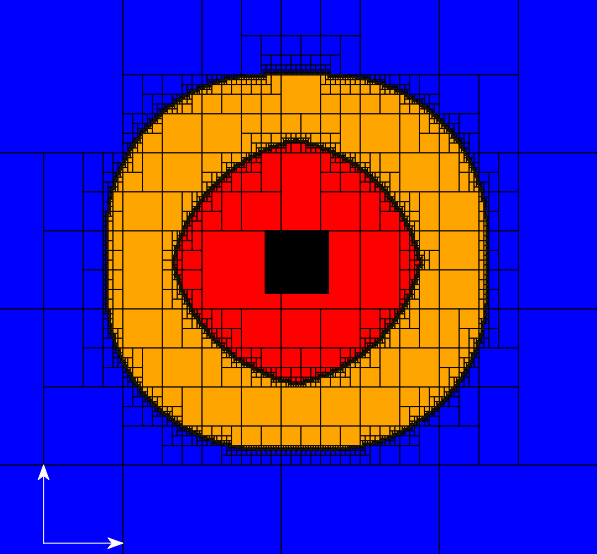
\includegraphics[scale=0.6,angle=0]{1_boat_efficient_border.png}
    \caption{Zone secured by one boat in red, orange zone is uncertain, yellow is the border and blue is not secured.}
    \label{fig:SecureZoneMAYBEOneBoat}
\end{figure}

Now that the algorithm is working for on boat, other can be added:

\begin{figure}[H]
\centering
    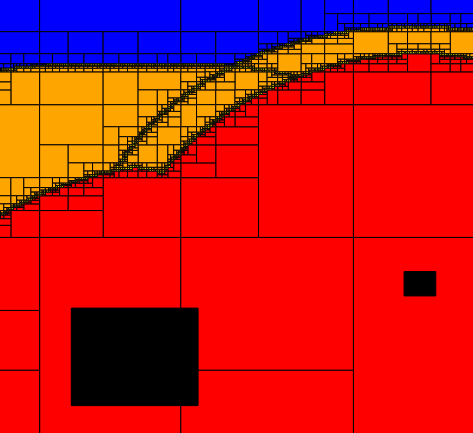
\includegraphics[scale=0.9,angle=0]{2_boat_overwriting_border.png}
    \caption{Zone secured by two boat in red, orange zone is uncertain, yellow is the border.}
    \label{fig:SecureZoneTwoBoat}
\end{figure}


The table shown earlier was not completely correct, as it was omitting the overlapping of the different boats as seen in the figure~\ref{fig:SecureZoneTwoBoat}, the external border of the zone covered by on boat is overlapping the uncertain zone of a different boat.\newline

In order to avoid those wrong and useless computations, the algorithm~\ref{alg:one_boat_alg} need to take into account the fact that an external border for a boat can be in an uncertain zone of an another boat, this change the correspondence table to:

\begin{center}
\begin{tabular}{|m{0.10\linewidth}|m{0.15\linewidth}|m{0.5\linewidth}|}
\hline
 Symbol & In Algorithm  & Meaning  \\ \hline
 0 & OUT & Box is not in the Secure Zone  \\ \hline
 1 & IN & Box is in the secure zone \\ \hline
 ? & UNKNOWN & Box is at the border of the secure zone  \\ \hline
[0,?]& UNKNOWN2  & Box is on the external border of the covert zone \\ \hline
[?,1]& UNKNOWN  & Box is on the internal border of the covert zone\\ \hline
[0,1]& MAYBE  & Box is in the uncertainty zone\\ \hline
   
\end{tabular}
\end{center}

Now the algorithm~\ref{alg:one_boat_alg} need to update this is done by changing the return from UNKNOWN to UNKNOWN2 in operand~\ref{op0}.\\
But the result seen in figure~\ref{fig:SecureZoneTwoBoat} need to fusion result of algorithm~\ref{alg:one_boat_alg} between the different boat,  this can be done by evaluating the result two by two boats, which correspond to the Truth table that follow:

\begin{center}
\begin{tabular}{|m{0.20\linewidth}|m{0.07\linewidth}|m{0.07\linewidth}|m{0.07\linewidth}|m{0.07\linewidth}|m{0.07\linewidth}|m{0.07\linewidth}|}
\hline
Test1/Test2 & 0 & 1 & ? & [0,?] &  [?,1] & [0,1] \\ \hline
          0 & 0 & 1 & ? & [0,?] &  [?,1] & [0,1]  \\ \hline
          1 &   & 1 & 1 &   1   &    1   &   1  \\ \hline
          ? &   &   & ? &   ?   &  [?,1] & [?,1] \\ \hline
      [0,?] &   &   &   & [0,?] &  [?,1] & [0,1] \\ \hline
      [?,1] &   &   &   &       &  [?,1] & [?,1] \\ \hline
      [0,1] &   &   &   &       &        & [0,1]  \\ \hline   
\end{tabular}
\end{center}

This truth table is translated in an algorithm(see~\ref{alg:fus_boat_alg}).

\begin{algorithm}[H]
\caption{Is $\mathbf{X} \subseteq \mathbb{S}$ , $\mathbb{S} =$ Secure Zone and $\mathbf{X} \in \mathbb{R^{\textnormal{\ensuremath{2}}}}$ }
\label{alg:fus_boat_alg}
\begin{algorithmic}[1]
\REQUIRE $X$,$range $ (reach of a boat),$M$ (list of position of boats)
\STATE $R \leftarrow \{\textnormal{Algorithme$~\ref{alg:one_boat_alg}
$(X,range,m)}\}_{m\in M}$
\IF{$\textnormal{IN} \subset R$}
\RETURN $\textnormal{IN}$
\ELSIF {$\textnormal{UNKNOWN} \subset R $}
\RETURN $\textnormal{UNKNOWN}$
\ELSIF {$\textnormal{MAYBE} \subset R $}
\RETURN $\textnormal{MAYBE}$
\ELSIF {$\forall r \in R $, $ r = \textnormal{OUT} $}
\RETURN $\textnormal{OUT}$
\ELSE
\RETURN $\textnormal{UNKNOWN}$
\ENDIF
\end{algorithmic}
\end{algorithm}

\begin{figure}[H]
\centering
    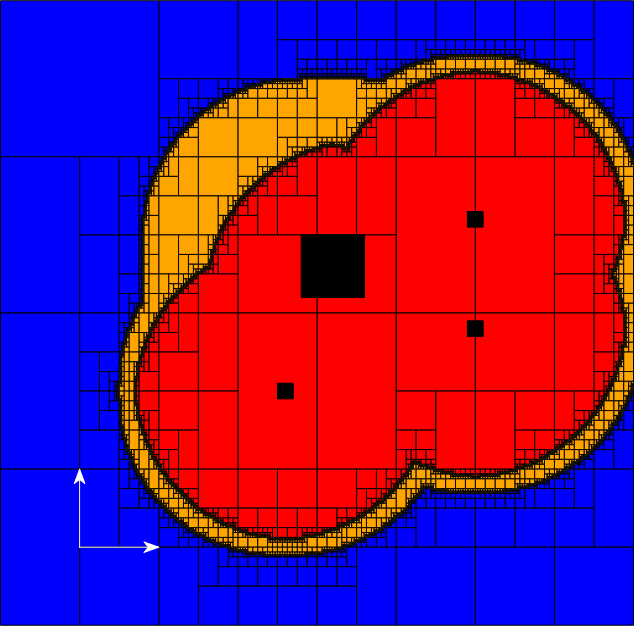
\includegraphics[scale=0.6,angle=0]{4_boat_right_border.png}
    \caption{Zone secured by four boat in red, orange zone is uncertain,blue is not secured.}
    \label{fig:SecureZoneFourBoat}
\end{figure}


Those last changes make the computation of the zone more efficient and correct, in figure~\ref{fig:SecureZoneFourBoat} there is no more overlapping of the external border.\\
If the uncertain zone is not needed the computation of the algorithm SIVIA can be accelerated by ignoring it. This can be done by changing the return value in the operand~\ref{op0} in the algorithm~\ref{alg:one_boat_alg} from UNKNOWN2 to OUT and the return value in the operand~\ref{op1} from MAYBE to OUT (the second change will not improve efficiency but just place the box in the right set), the result can be observed in figure~\ref{fig:SecureZoneFourFastBoat}.

\begin{figure}[H]
\centering
    \begin{minipage}[b]{0.4\textwidth}
    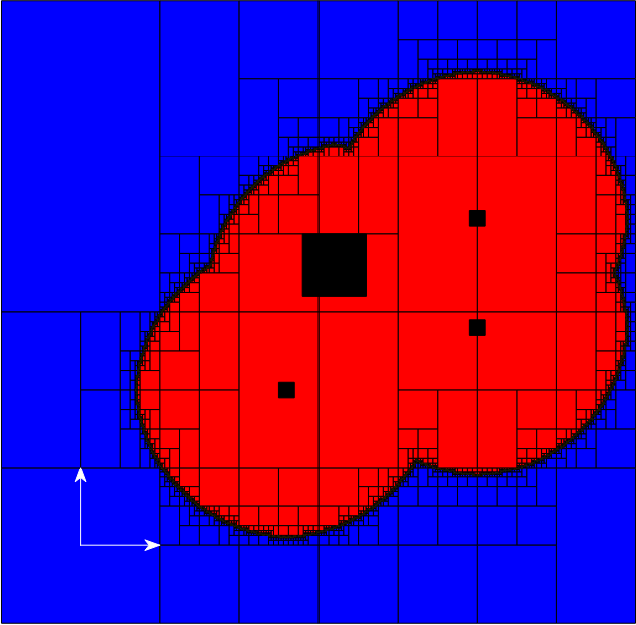
\includegraphics[scale=0.4,angle=0]{4_boat_right_border_fast_comp.png}
    \caption{Zone secured by four boat computed with algorithm ~\ref{alg:fus_boat_alg} and ~\ref{alg:one_boat_alg}.}
    \label{fig:SecureZoneFourFastBoat}
    \end{minipage}
    \begin{minipage}[b]{0.4\textwidth}
    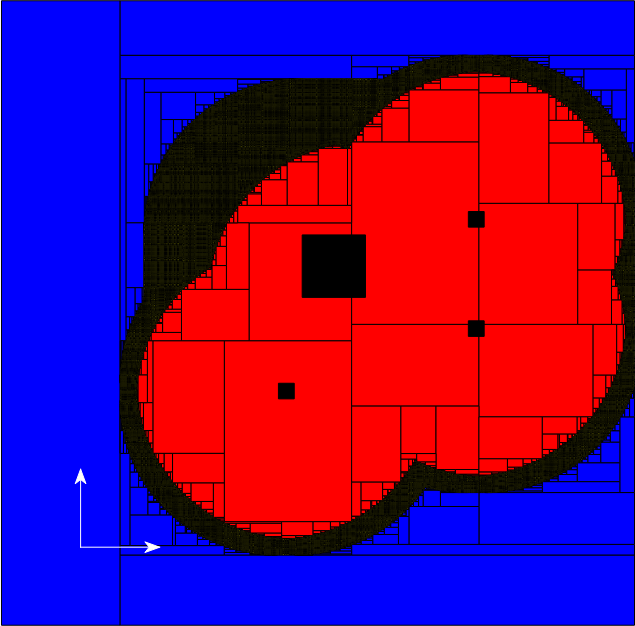
\includegraphics[scale=0.4,angle=0]{4_boat_right_border_sep_comp.png}
    \caption{Zone secured by four boat computed with separators}
    \label{fig:SecureZoneFourSepBoat}
    \end{minipage}
\end{figure}

The result in figure~\ref{fig:SecureZoneFourFastBoat} may also be obtain with the combination of separators (see figure~\ref{fig:SecureZoneFourSepBoat} but the result will be longer to get as it have to cut through the uncertain zone even if it is time consuming (and with no information gain). To demonstrate the waste of time done by the separators the figure~\ref{fig:SecureZoneFourSepBoat} has taken thirty six times the time taken to compute the figure~\ref{fig:SecureZoneFourFastBoat} (fastest computation times).

\section{Map generation and origin estimation}

\textcolor{blue} {\textit{Khadimoullah Vencatasamy}}

We want to simulate on a map and we want to generate the map easily. So the easiest way we found was to take a screen on Google earth where we know the scale.
Our objective is to transform this map into a binary image. To do so we choose to make a color filter to isolate the ground from the sea. We thought to use a contour filter but due to the many bumps present on the satellite view sea it was successful.

So we have a script which take a satellite view as input, when you run this script you have to windows: one with some trackbar which you can slide to filter the color you want and apply a closing filter  to erase the last parasite pixels. The second window show the output image. Press 's' to save the output image.

\begin{figure}[H]
\centering
  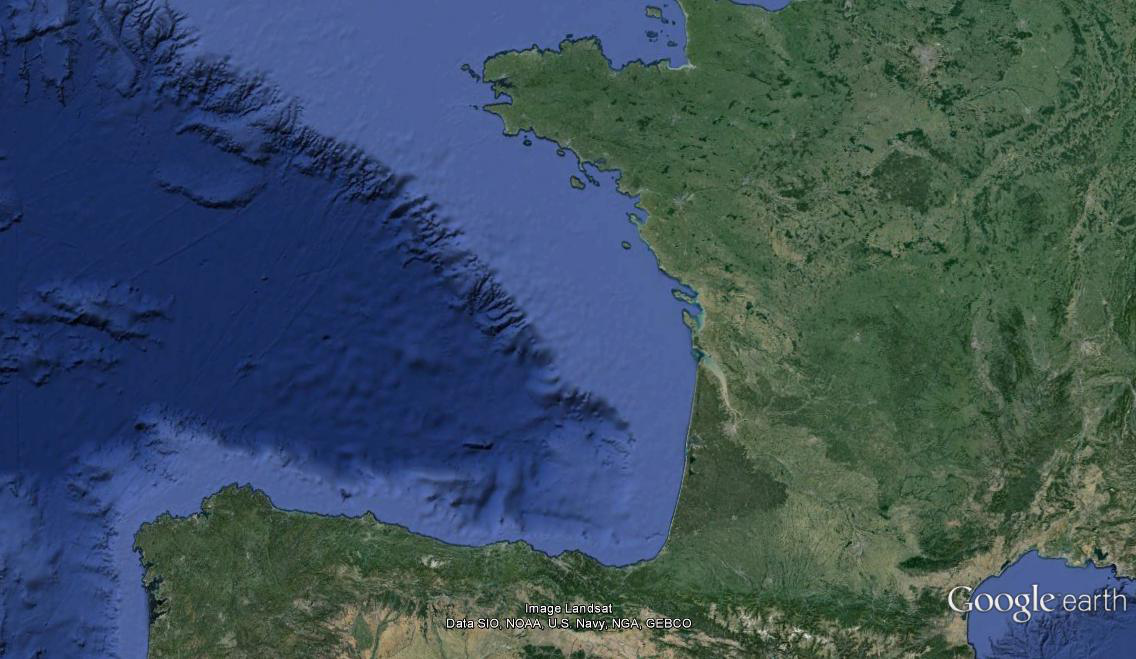
\includegraphics[width=0.6\linewidth]{GascogneSat.png}
  \caption{Input Image}
\end{figure}

\begin{figure}[H]
\centering
  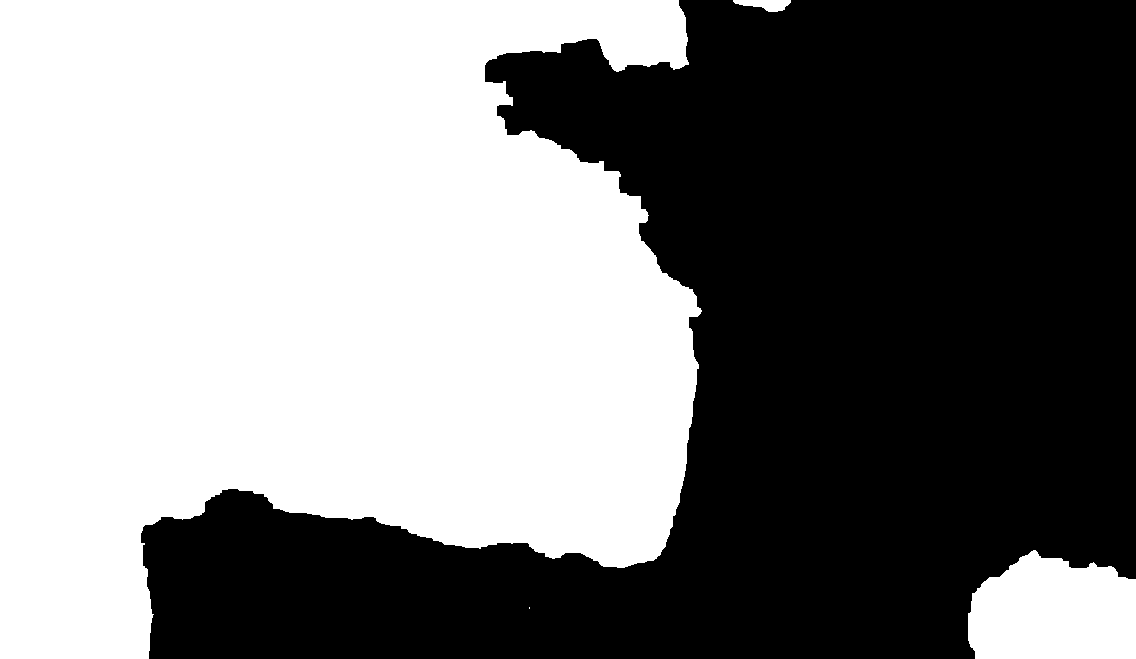
\includegraphics[width=0.6\linewidth]{BWFrance.png}
  \caption{Output Image}
\end{figure}


\begin{figure}[H]
\centering
  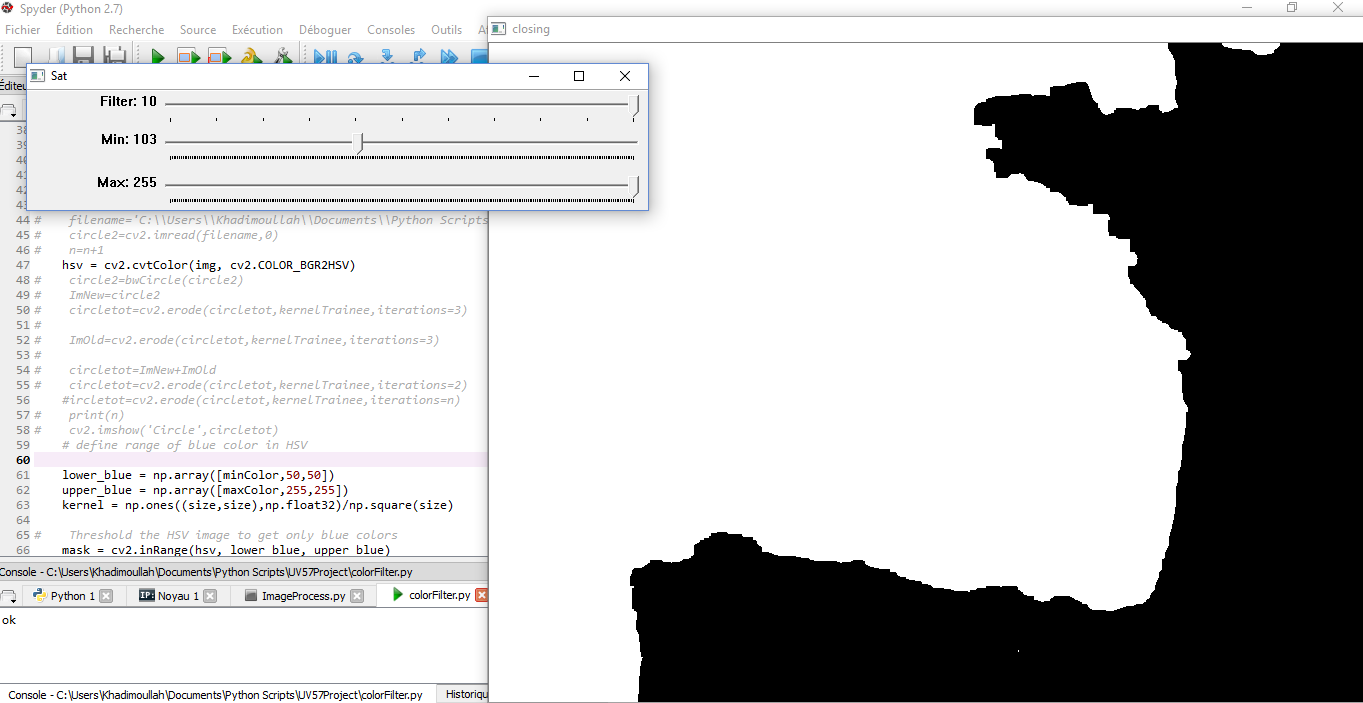
\includegraphics[width=0.6\linewidth]{BWFranceInterface.png}
  \caption{Interface to binarize the satellite image}
\end{figure}

This is this image which is use to generate the paving in ImageToBoxes script.

\subsection{Origin Determination}

In our problem we set the origin of the map to the point 45$^\circ$N 4$^\circ$W so we need to find the (i0,j0) which are the coordinates of the origin.

To achieve this we need the latitude and the longitude of the top left corner of our binary map.
We will note X Y for the coordinate in pixel and LAT LONG for the coordinate in WPs.

First let's determine the $\delta{X}$ and $\delta{Y}$:

%\begin{equation}
%\begin{case}
%\delta{X}=\frac{LONG2-LONG1}{X2-X1} & \text{ where LONG2 is the leftmost point and LONG1 is the rightmost point X1 and X2 is their X coordinate in pixel}\\
%\delta{Y}=\frac{LAT2-LAT1}{Y2-Y1} & \text{ where LAT2 is the	topmost point and LAT1 is the bottommost point Y1 and Y2 is their Y coordinate in pixel}\\
%\end{cases}\\
%\text{Lat0 and Long0 is the coordinate of the 0 0 pixel}\\
%\begin{case}
%LAT0=LAT1 -Y1 * \delta{Y} \\
%LONG0=LONG1 -X1 * \delta{X}\\
%\end{case}\\
%\text{We can now convert LAT/LONG to their pixel coordinate}\\
%\begin{case}
%X= \frac{LONG-LONG0}{\delta{X}}\\
%Y= \frac{LAT-LAT0}{\delta{Y}}\\ 
%\end{case}
%\end{equation}

In our case we have chosen (45$^\circ$N,4$^\circ$W) as origin which corresponds to the point (410 400) in pixel coordinate.



\section{Mesh to boxes functions}
\vspace{0.5 cm}
\textcolor{blue} {\textit{Maël LE GALLIC}}
\vspace{0.3 cm}

In order to define the \emph{Bay of Biscay}, $\mathbb{G}$, we have to implement a SIVIA test that distinguish the earth from the sea. To deals with it, we realised a procedure which returns the sub-pavings of an input binary image. 
First of all, we compute the integral image of the binary image. The integral image (or summed area table) is a data structure which permit to quickly and efficiently generate the sum of pixel values in a rectangular subset of an image. The value at any pixel (i, j) in the integral image correspond to the sum of all the pixels above and to the left of (i, j). To compute the sum of pixel values of a rectangular subset of the image only four pixel values of the integral are required. Hence, the calculation time is constant and independent of the size of the rectangular area. This sum of i(i,j) over the rectangle spanned by A, B,C and D is:

equation

\begin{figure}[!h] 
\center
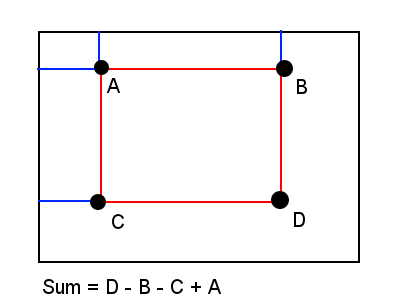
\includegraphics[scale=0.4]{integralImage.png} 
\caption{Description of computing a sum in an integral image } 
\label{fig: Integral image}
\end{figure}

Then, we use this integral image in our SIVIA test to say if the tested box is inside the 0-bit area, the 1-bit area or overlaps the two areas of the binary image. The procedure of the test is described below:
\begin{itemize}
\item We calculate the indexes of the four pixels corresponding to the vertices of the box.
\item We compute the number of pixel in the box: nbsPixel
\item By using the integal image, we compute the sum of pixel values in the box: sumPixel 
\end{itemize}
%\begin{algorithm}[H]
%\caption{SIVIA Test ImageToBoxes}
%\label{alg:one_boat_alg}
%\begin{algorithmic}[1]
%\REQUIRE $X$,$IntegralImage$\\
%1. We calculate the indexes of the four pixels corresponding to the vertices of the box.
%2. We compute the number of pixel in the box: nbsPixel
%3. By using the integal image, we compute the sum of pixel values in the box: sumPixel
%\IF \textnormal{$sumPixel == 0$}\\
%\RETURN \textnormal{$OUT$}\\
%\ELSIF \textnormal{$sumPixel == nbsPixel$} 
%\RETURN \textnormal{$IN$}
%\ELSE
%\RETURN \textnormal{$UNKNOWN$}
%\ENDIF
%\end{algorithmic}
%\end{algorithm}
\vspace{1cm}
An example of the application of the SIVIA algorithm with the ImageToBoxes test is shown below. In input we have a binary image of the Biscay Bay and in output the resulting sub-pavings.
\begin{figure}[H]
\centering
    \begin{minipage}[b]{0.4\textwidth}
    
\includegraphics[scale=0.4]{Gascogne2.png}
	\caption{Binary image of the Biscay Bay } 
	\label{fig: Biscay Bay}
    \end{minipage}
    \begin{minipage}[b]{0.4\textwidth}
    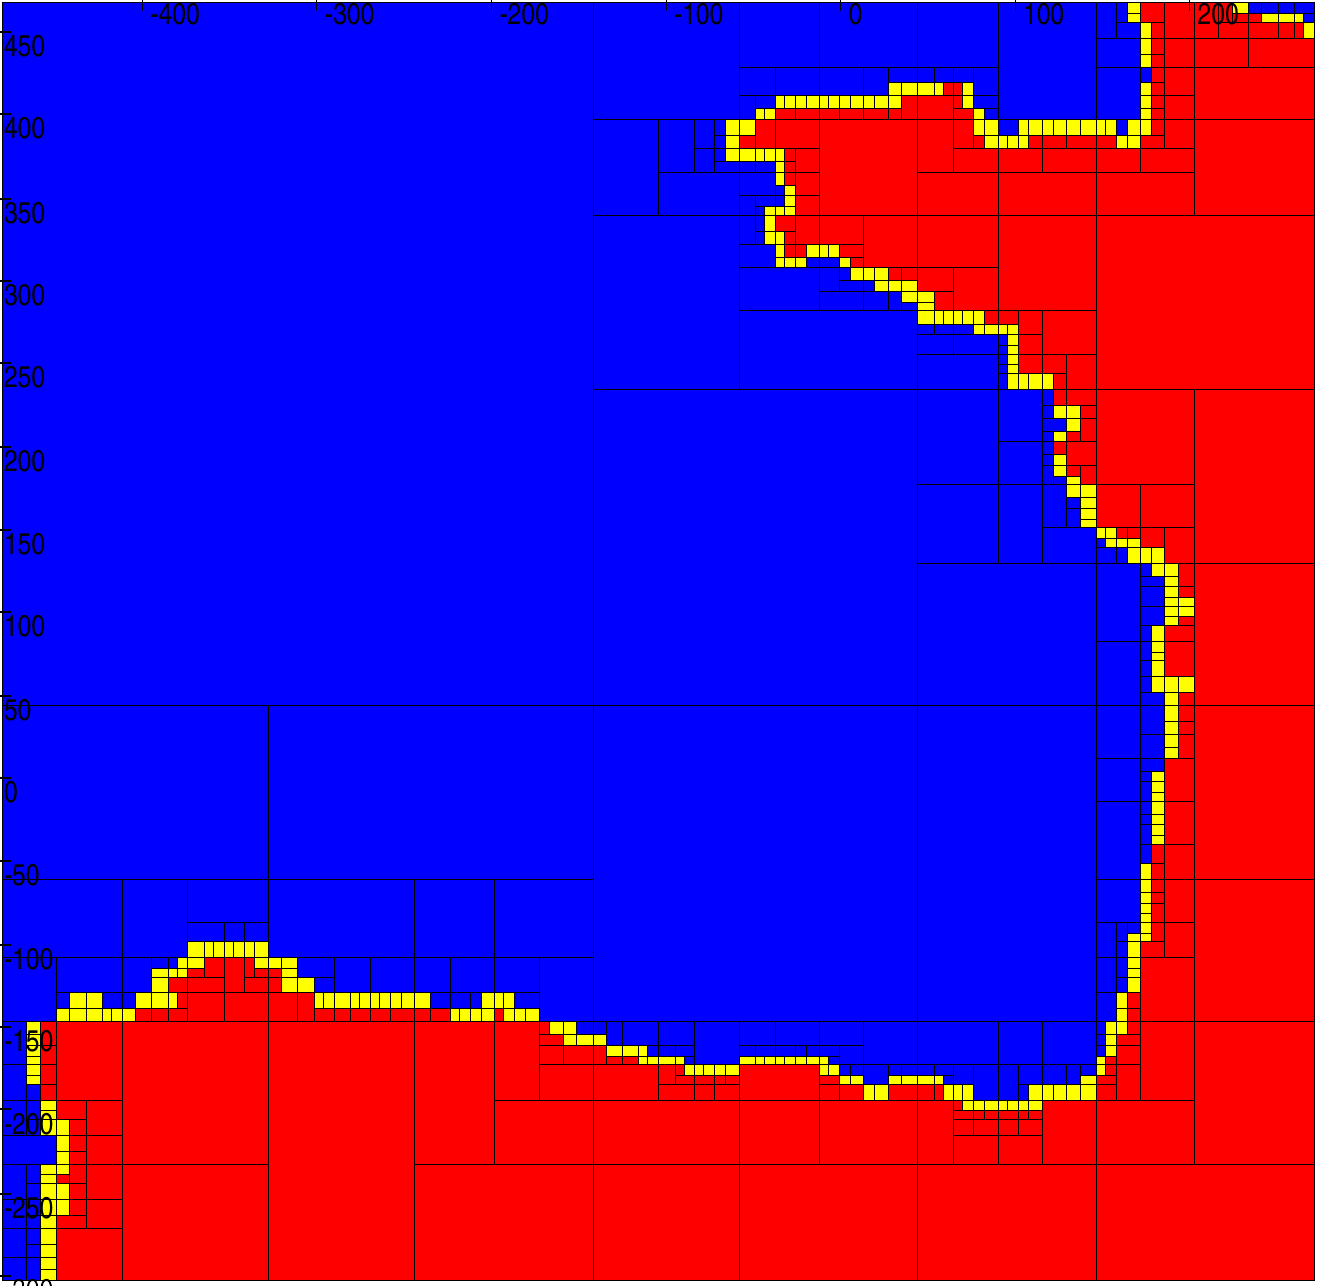
\includegraphics[scale=0.2]{GascogneBoxes.png} 
	\caption{Resulting sub-pavings of the Biscay Bay } 
	\label{fig: Sub-pavings of the Biscay Bay}
    \end{minipage}
\end{figure}



\section{Erosion functions}
\vspace{0.5 cm}
\textcolor{blue} {\textit{Khadimoullah Vencatasamy}}
\vspace{0.3 cm}
\subsection{Trail Modelization}

We have define the secure zone with this equation:\\
\begin{equation}
\mathbb{X}(t)=\mathbb{G}\cap\mathbb{F}_\delta(\mathbb{X}(t-\delta))\cap\bigcap\limits_{i \leq}((g_(a_i))^-1(d_i(t),\infty)))\\
\end{equation}

Where $\mathbb{F}_\delta(\mathbb{X}(t-\delta))$ represents the past of the secure zone. In fact, we can associtae that to the trail of our robot. 
To compute the trail we have got to solutions. The first one was to stock the positions of our robot and then generate virtual robot with a smaller field of view. But with this solution we need to compute a lot ressources in interval analysis. So the second idea was to apply an erosion on an image. So we do not have to compute interval analysis. Then we give this new image with the trail to the script ImageToBoxes saving a lot of time of calculation.

\begin{figure}[H]
\begin{center}
  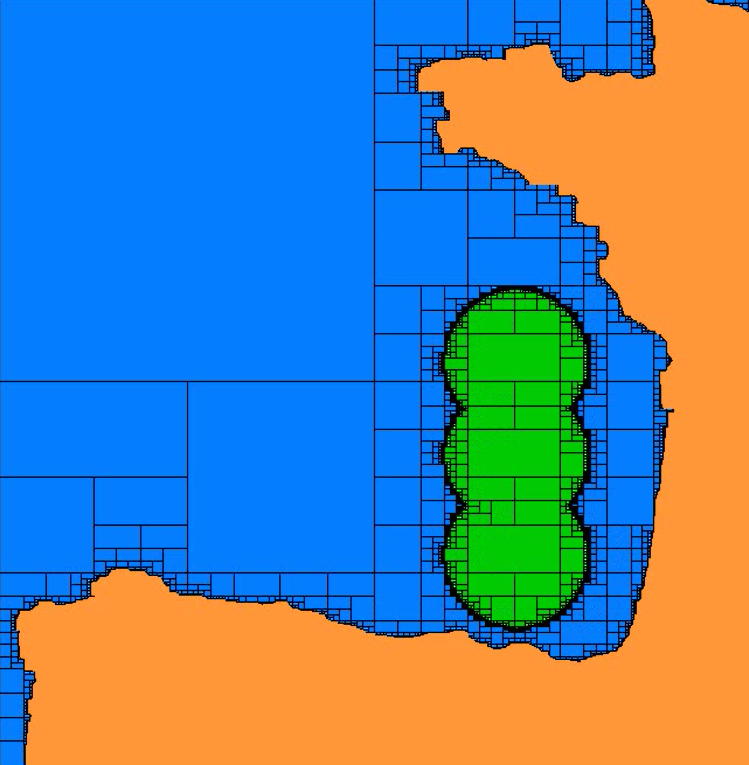
\includegraphics[width=0.6\linewidth]{WithoutTrail.png}
  \caption{Robot without}
\end{center}
\end{figure}


\begin{figure}
\begin{center}
  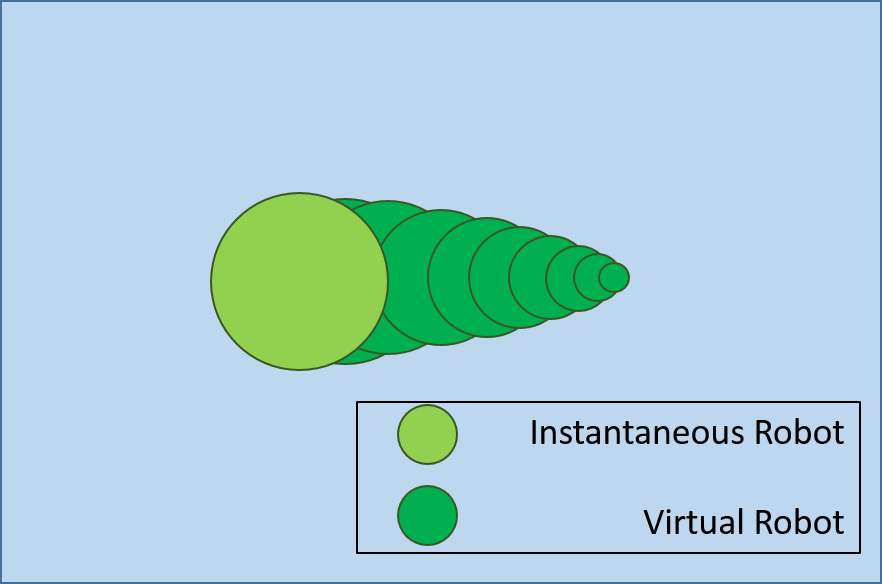
\includegraphics[width=0.6\linewidth]{TrailVirtualRobot.png}
  \caption{Trail Implementation with erosion}
\end{center}
\end{figure}

Finally, the erosion allow us to conclude if our algorithm is efficient. In fact, when the swarm covers the Bay of Biscay, even if a little zone is not covered the erosion will expand this area.

\begin{figure}[H]
\begin{center}
  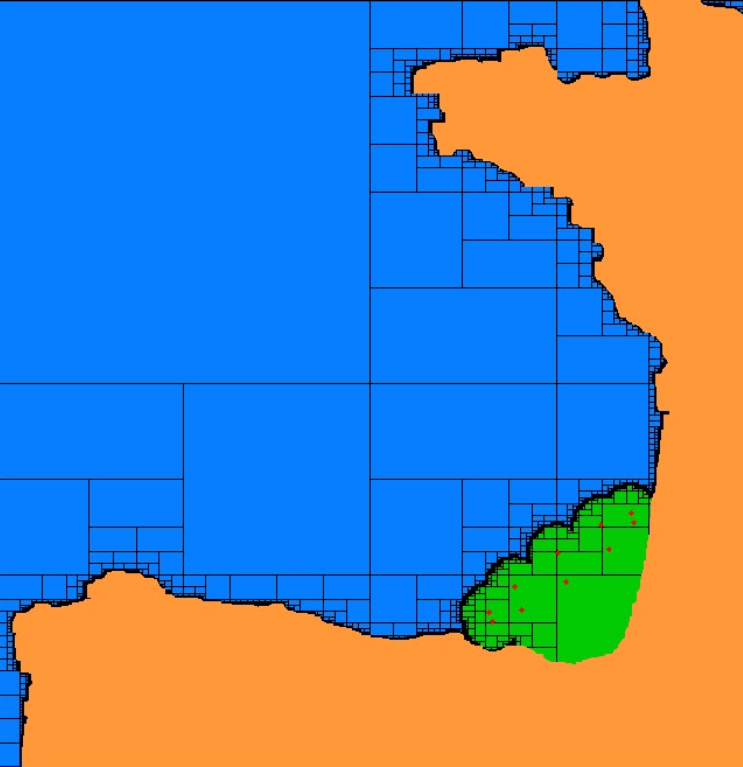
\includegraphics[width=0.6\linewidth]{FailZone.png}
  \caption{The swarm misses a little area}
\end{center}
\end{figure}

\begin{figure}
\begin{center}
  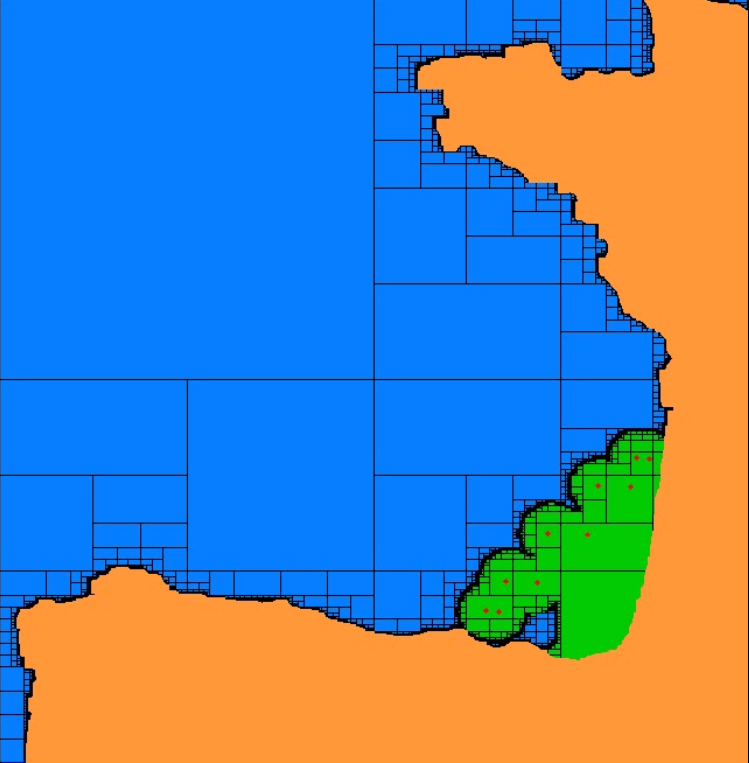
\includegraphics[width=0.6\linewidth]{FailZoneExpand.png}
  \caption{The uncovered area is expanded due to the erosion}
\end{center}
\end{figure}



\section{Global Sivia algorithm}

\section{SIVIA Algorithm}

\vspace{0.3 cm}
	
	\textcolor{blue} {David DUVERGER}
	
	\vspace{0.5 cm}
	
	We will present here the fusion of the paving of the Gascogne Golf, the robots and their erosion. So, it is the resolution of the following mathematical formula:
	
	$$X(t) = G \cap F_{\delta}(X(t-\delta)) \cap g^{-1}([di,\infty])$$
	

\begin{algorithm}
  \caption{SIVIA algorythm}
  \vspace{0.5 cm}
  \textbf{Inputs}% Inputs section
  \begin{algorithmic}[1]
    \STATE Area $X0$
    \STATE Object $France$
    \STATE Object $Erosion$
    \STATE Object $Robots$
    \STATE Float $Precision$
  \end{algorithmic}
  \bigskip

  \textbf{Output}% Output section
  \begin{algorithmic}[1]

    \STATE Boxes $France U Robots U Erosion$
    \STATE Boxes $Robots U Erosion$
    \STATE Boxes $Sea$
  \end{algorithmic}
  \bigskip
  
  \textbf{Initialization}% Initialization section
  \begin{algorithmic}[1]
   	\STATE $stack\gets X0$
	\STATE $BoxesFranceURobotsUErosion\gets []$
	\STATE $BoxesRobotsUErosion\gets []$
	\STATE $BoxesSea\gets []$
  \end{algorithmic}
  
\end{algorithm}




\newpage


\begin{algorithm}
  \caption{SIVIA algorythm (continued)}
  \begin{algorithmic}
	\WHILE{len of stack >0}
	
		\vspace{0.3 cm}
	
  		\STATE $X\gets Interval \hspace{0.1cm} Vector \hspace{0.1cm} of \hspace{0.1cm} stack$
		\STATE $FranceTest\gets France.function(X)$
		\STATE $ErosionTest\gets Erosion.function(X)$ 
		\STATE $RobotsTest\gets Robots.function(X)$

		\vspace{0.3 cm}

  	 	\textcolor{blue}{//If we are in the France, robots or erosion:}\
	 	
	 	\IF{FranceTest==IBOOL.IN or ErosionTest == IBOOL.IN or RobotsTest == IBOOL.IN}
     	  	\STATE $Add \hspace{0.1cm} X \hspace{0.1cm} to \hspace{0.1cm} BoxesFranceURobotsUErosion$
     	
	 	\vspace{0.3 cm}
	 	
	 	\textcolor{blue}{//If we are in the robots or erosion:}\
	 	 \IF{RobotsTest == IBOOL.IN or ErosionTest == IBOOL.IN}
     		\STATE $Add \hspace{0.1cm} X \hspace{0.1cm} to \hspace{0.1cm} BoxesRobotsUErosion$
	 	 
	
	 	 \ENDIF
	 	 
	 	 \vspace{0.3 cm}
     		
     	\textcolor{blue}{//Else if we are outside all:}\
	 	 \ELSIF{ $FranceTest == IBOOL.OUT \hspace{0.1cm} and \hspace{0.1cm}  ErosionTest == IBOOL.OUT \hspace{0.1cm} and \hspace{0.1cm}  RobotsTest == IBOOL.OUT$}
	 	 \STATE $Add \hspace{0.1cm} X \hspace{0.1cm} to \hspace{0.1cm} BoxesSea$
	 	 
     	\ELSE
     
      	\vspace{0.3 cm}
     			\IF{Size \hspace{0.25cm} of \hspace{0.1cm} X > Precision}
          			\STATE $(X1, X2)\gets cut \hspace{0.3cm}  X$
          			\STATE $Add \hspace{0.3cm}  X1 \hspace{0.3cm}  in \hspace{0.3cm}  stack$
         			\STATE $Add \hspace{0.3cm}  X2 \hspace{0.3cm}  in \hspace{0.3cm}  stack$
         		\ENDIF
         	
  		\ENDIF
  		 \vspace{0.3 cm}
 	 \ENDWHILE 
	
	\vspace{0.3 cm}
	
  return BoxesFranceURobotsUErosion,BoxesRobotsUErosion,BoxesSea


  \end{algorithmic}
\end{algorithm}


\clearpage



\newpage

	With the help of this algorythm we can have a paving of the intersection between the Gascogne Golf, the robots and their erosion. We arrive to obtain the following result:
	

	
	\begin{figure}[!h] 
    \center
    	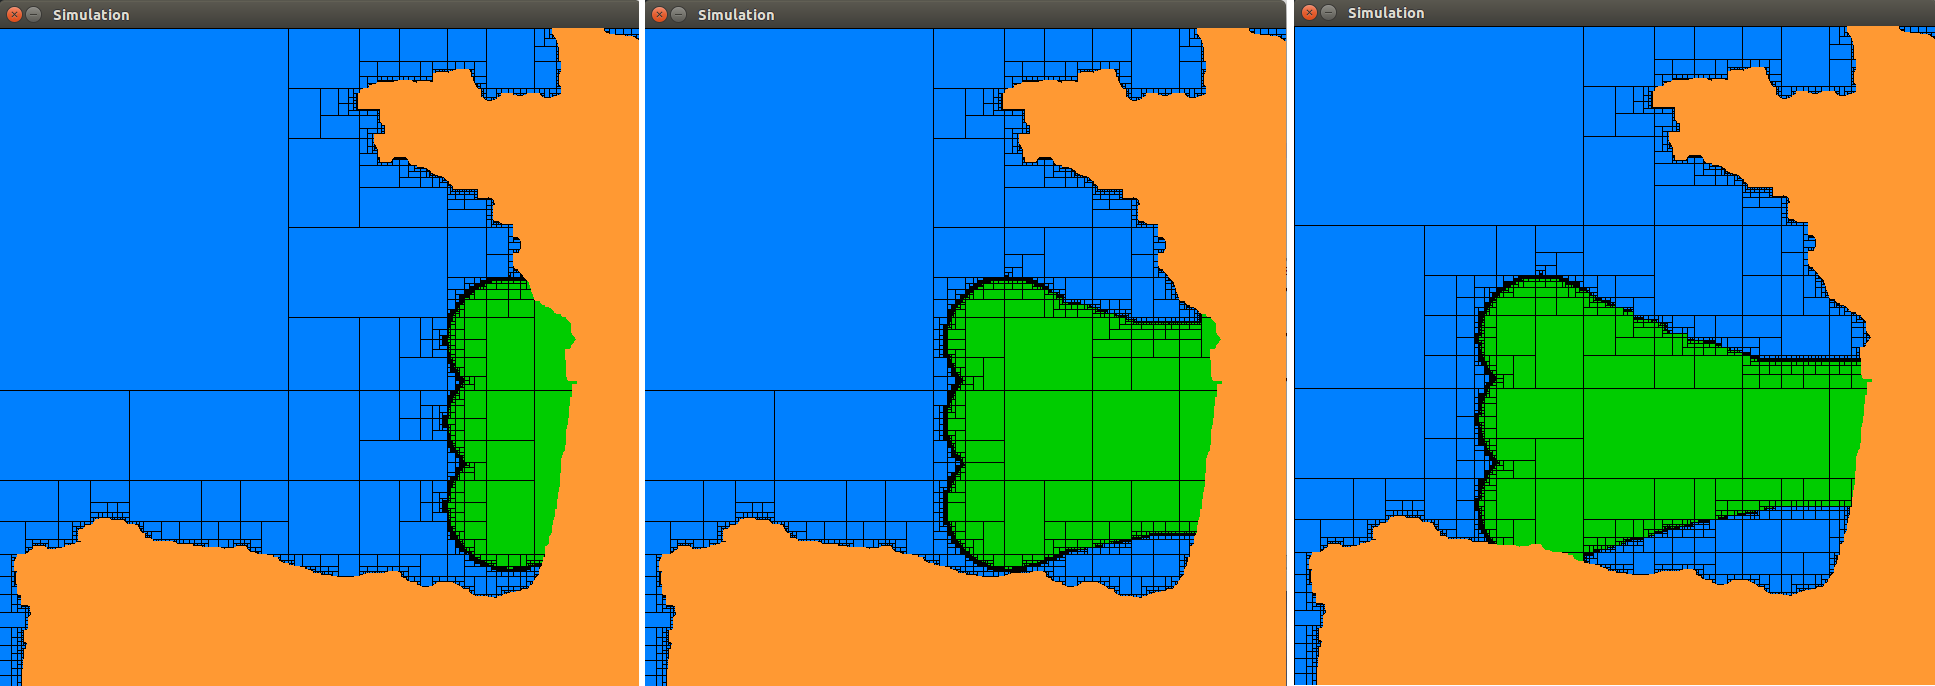
\includegraphics[scale=0.25]{SimulationFusion.png} 
    	\caption{Paving of the intersection between the Gascogne Golf, the robots and their erosion } 
    \label{S1 U S2}
	\end{figure} 


\section{Results}

\paragraph{Distribution of the robots}

At first we thought about distributing the robots with a regular spacing along the curvilinear abscissa of the ellipse. This method being too difficult in terms of mathematical theory as well as algorithmical means, this solution was abandoned. In fact, we should have approximated the Wallis' integrals to a limited development which is quite prickly. This would have implied a long programming time and a processing time too lengthy for a simple feasibility study.\\

That is why we decided to forget this method in benefit for an easier one which involves angular delays. Thus, each robot follows the previous one with a given angular delay depending on how many robots there are covering the ellipse.
This implies that the nearer the robots are to the apogees, the nearer they will be with one another and on the contrary, the nearer they are to the perigees, the farer they are with one another. However, the non linearity in terms of distance between every robots does not impede the conservation of the secure zone. As a matter of fact the robots are faster when they are near the perigee. Therefore the streaks are bigger and so fill in the gaps between the robots. This way we can guarantee the continuity of the secure zone the robots are watching over.//





%----------------------------------------------------------------------------------------
%	PART III 
%----------------------------------------------------------------------------------------
\chapter{Robots regulation}

\section{Regulation}
Two methods have been studied and implemented to regulate the pack of robots. The first approach is a method based on artificial potentials field. This method is robust and easy to debug. It was chosen to regulate the real robots on the testing field because it was easier to implement on the robots and provided good results. The second one is a method of feedback linearisation. This method was chosen for the simulation of the surveillance of the Bay of Biscay because it is a classic and efficient method.

\subsection{Artificial Potentials Field}
\vspace*{0.5 cm}
\textcolor{blue} {Thomas Boulier \& Sylvain Hunault}
\vspace*{0.5cm}

Let $p_{robot}$ be the position of our considered robot, let $p_{target}$ and $v_{target}$ be the position and speed of the target we want the robot to reach.
We can consider the robot and the target as two particles of opposite charge, and then compute the potentials field between them. In case of obstacles, we can consider them as particles of same charge than the robot's.
The potentials field method calculates the instantaneous speed vector $w(p_{robot},t)$ the robot needs to reach (or at least follow) the target. To compute that speed, we use the potential $V$ between the robot and the target :\\
\[ V(p_{robot}) = v^T_{target}. p_{robot} + \|p_{robot}-p_{target}\|^2 \]
And compute the gradient of that potential to find the order $w(p_{robot},t)$:
\[w(p_{robot},t) = -grad(V(p_{robot})) = -\frac{dV}{dP}(p)^T\]
So :
\[w(p_{robot},t) = v_{target}-2.(p_{robot}-p_{target})\]
For $w$, we compute the order speed and course:
\[\bar{v} = \|w\| \]
\[\bar{\theta} = tan(\frac{w_y}{w_x})\]

As illustrated in the picture below, a proportional regulation computes the command $u_v$ and $u_{\theta}$ which will be used to control the robot.

\[ u_v = Kp_v \cdot (\bar{v}-v_{robot}) \]
\[ u_{\theta} = Kp_{\theta} \cdot (\bar{\theta}-\theta_{robot}) \]

Where $\theta_{robot}$ is the course of the robot calculated by finite difference because the GPS of the robot do not provide the course.

\begin{figure}[H]
   \caption{\label{schema_regulation_potentiels} Architecture of the potentials field method}
   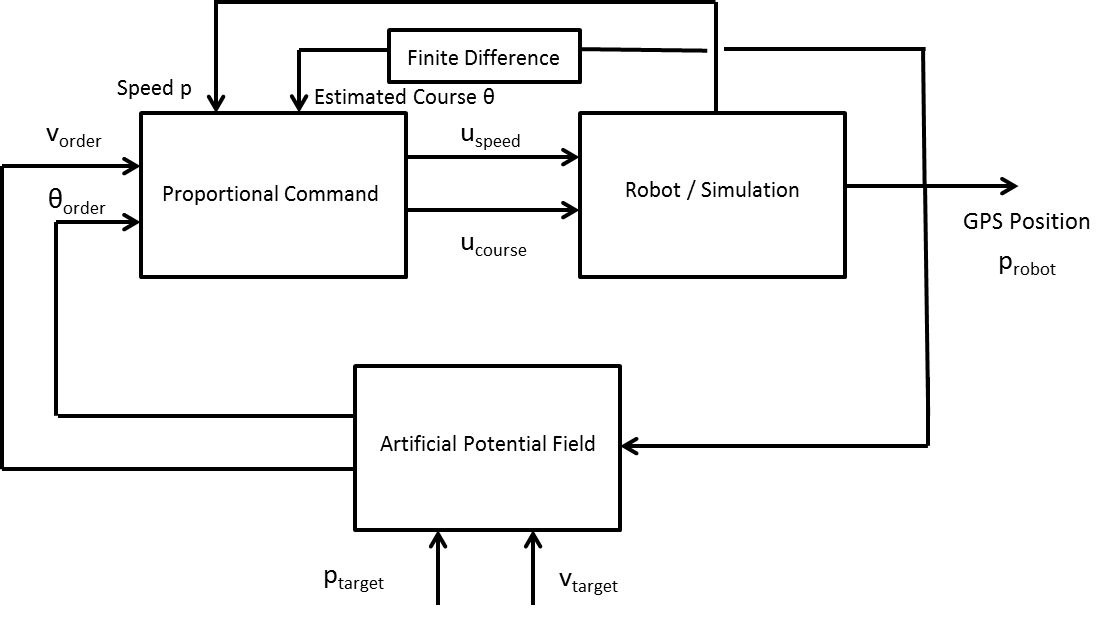
\includegraphics{schema_regulation_potentiels.png}
\end{figure}

$u_v$ and $u_{\theta}$ are saturated to avoid an overloading of the actuators.\\

This command is then used as the entry of a simple simulator used to test the regulation.
The command is used as the acceleration of the robot, and its position at each time is computed through an Euler method. The objective point is on an parametric ellipse moving with time.\\

The method is easily extended to multiple robots : each one is controlled separately. For each iteration of the loop, the regulation process is applied on each robot. The command is calculated for each one, then the simulation uses it to compute the new position of each one.

$u_v$ and $u_{\theta}$ are saturated to avoid a surcharge of the actuators. 

\subsection{Feedback Linearisation}
\vspace*{0.5 cm}
	\textcolor{blue} {Alice Danckaers}
\vspace*{0.5cm}

Feedback linearisation is a classical approach used in controlling nonlinear systems. We transform the nonlinear system \ref{system1} into an equivalent linear system \ref{system2}, which is of the form $\ddot{y}=A(x)*u$.

\begin{equation}
\dot{x} = f(x,u) \rightarrow \left\{ 
\begin{array}{l l}
  \dot{x_1} = x_4 * \cos(x_3)\\
  \dot{x_2} = x_4 * \sin(x_3)\\
  \dot{x_3} = u_1\\
  \dot{x_4} = u_2\\
\end{array} \right.
\label{system1}
\end{equation}

\begin{equation}
\begin{pmatrix}
	\ddot{y_1}\\
	\ddot{y_2} 
\end{pmatrix}
=
\begin{pmatrix}
	-x_4*\sin(x_3) & \cos(x_3)\\
	 x_4*\cos(x_3) & \sin(x_3)
\end{pmatrix}
\begin{pmatrix}
	u_1\\
	u_2
\end{pmatrix}   
\hspace*{1cm} \textnormal{ with } y = \begin{pmatrix}
	x_1\\
	x_2
\end{pmatrix}
\label{system2}
\end{equation}

If $w$ is the instruction of the robot has to follow, then we have the expression of $u$ as shown in equation \ref{equationU}. We can then use it to regulate the robot in an Euler method.
\begin{equation}
 u =
\begin{pmatrix}
	-x_4*\sin(x_3) & \cos(x_3)\\
	 x_4*\cos(x_3) & \sin(x_3)
\end{pmatrix}^{-1}
\begin{pmatrix}
	(y_1-w_1) + (\dot{y_1} - \dot{w_1}) -  \ddot{w_1}\\
	(y_2-w_2) + (\dot{y_2} - \dot{w_2}) -  \ddot{w_2}
\end{pmatrix}
\label{equationU}
\end{equation}


\section{Evolution of the elliptic trajectory}
%\section{Evolution of the elliptic trajectory}
\textcolor{blue} {Rafael FINKELSTEIN \& Thiago OLIVEIRA RODRIGUES}


The goal of this part was to choose an approach to secure the Bay of Biscay with a configurable number of robots. The technique chosen was to dispose the robots around an ellipse and rotate and translate this ellipse in a way the robots would secure all the region of the bay until reach a final position.  The process to calculate the trajectory of each robot is divided in two basic parts. The first part is the evolution of ellipse’s parameters such as relative centre position, angle of inclination and ellipse’s major axe. The other part is the calculation of the ellipse and the robot’s position in it.
\vspace*{0.5cm}


In order to calculate the way points, the points where the ellipse path should pass through, it was chosen some GPS coordinates to be the extremal points of the ellipse, in other words, the closest that the robots will need to go to the coast. After the transformation of the extremal points from GPS coordinates to the system coordinates it is possible to geometrically calculate the ellipse’s parameters (x and y centre, inclination angle and major axe length).
\vspace*{0.5cm}


Knowing the way points, in each time step the ellipse grows and rotates linearly until it reaches the next way point. When the last way point is reached it means that all Bay of Biscay is secured and the robots keep moving around the last ellipse creating a barrier that makes impossible to pass through without entering the zone secured by some robot.
\vspace*{0.5cm}

To calculate the robot target position, each robot was disposed with an equal distance in between the others in the perimeter of a circle, in this circle it was applied the matrix of linear transformation and the rotation matrix. Those values are send to a log that in the field will be used to control the real robots.
\vspace*{0.5cm}

%\begin{figure}[!htb]
%	\begin{center}
%		\includegraphics[scale=0.4]{ellipse.png} 
%		\caption{\label{Evolution of the elliptic trajectory} Final ellipse}
%	\end{center}
%\end{figure}



\section{Conversion of the order to a PWM command}
The regulation process returns the two values ($u_v$,$u_{\theta}$) as ouput. But those values are in "natural" unit, which is acceptable for a simulation but not for the regulation of actual robots.
At the end of the regulation,the command is saturated, so the range of $u_v$ is [0,1] , while the range of $u_{\theta}$ is [-10,10].
The command needs to be transformed in an acceptable value for the robots.
the command taken by the robots is a PWM values in the range [1000,2000]. Because we need to keep the robots always moving, we do not want to allow the robots to have a null speed or worst, a negative one.
To ensure that, we maintain the forward command slightly over 1500. The turn command however needs to have the same degree of freedom below and beyond the neutral point of 1500.
So we linearly transform  ($u_v$,$u_{\theta}$) into a couple of PWM values, of range [1600,2000]\times [1000,2000]. 
We considered using a smoother transition than the linear transformation of a saturated command, such as the hyperbolic tangente, but we finally decided that it was not necessary.



%----------------------------------------------------------------------------------------
%	PART IV 
%----------------------------------------------------------------------------------------
\chapter{Implementation with buggy robots}
\section{Hardware}
\textcolor{blue}{\textit{Maxime Bouyssou}}



\subsection{Hardware architecture}
The hardware part of each robot is pretty simple. Each robot is equipped with a serial GPS wired to a serial radio module (see figure below). So each robots will emits its GPS coordinates to the central computer who will then uses this coordinates to compute the next order he will send to them.

\begin{center}
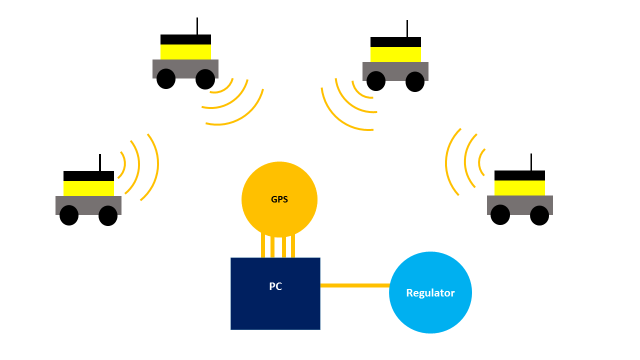
\includegraphics[scale=0.6]{GPS_emit.png} 
\captionof{figure}{Robot emitting their GPS coordinates}
\label{fig1}
\end{center}

The radio modules are wired to the power electronic parts of the robot. The robot is controlled via a standard RC radio link. The idea is that the central computer can directly send his orders via the radio transmission to the robots. (see figure below)

\begin{center}
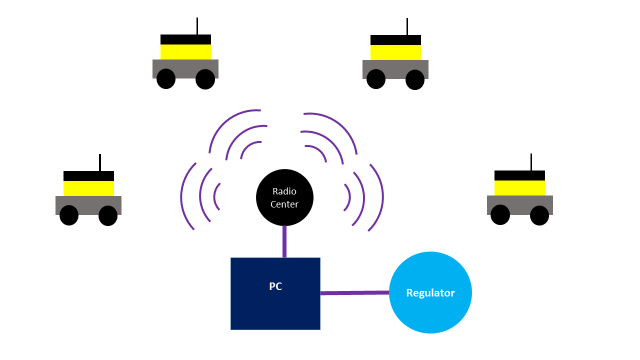
\includegraphics[scale=0.6]{Radio_control.png} 
\captionof{figure}{Robot emitting their GPS coordinates}
\label{fig1}
\end{center}

Here is a more details view of all the composants inside the robots.

\begin{center}
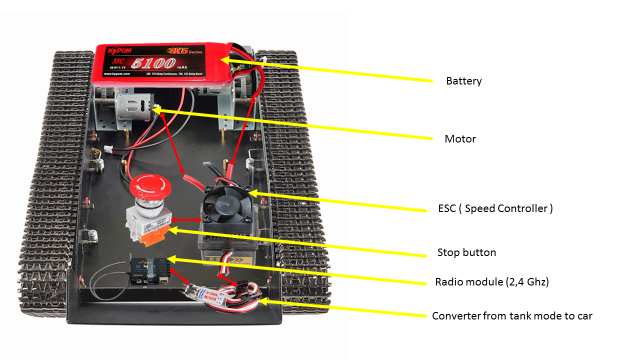
\includegraphics[scale=0.6]{robot.png} 
\captionof{figure}{Construction of the robot	}
\label{fig1}
\end{center}

Here is a more details view of all the composants on the ground station

\begin{center}
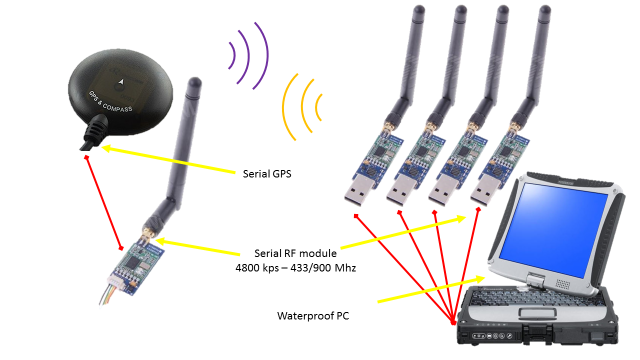
\includegraphics[scale=0.6]{GPS.png} 
\captionof{figure}{GPS}
\label{fig1}
\end{center}

\begin{center}
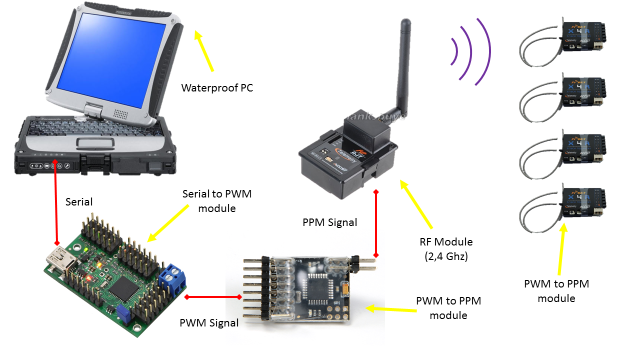
\includegraphics[scale=0.6]{stationControl.png} 
\captionof{figure}{Station Control}
\label{fig1}
\end{center}
\section{GPS Sentence Analysis}
\chapter{Réalisation de test sur robot char}
\section{Matériel}
\subsection{GPS}
ici la description des GPS utilisés
\subsection{Robot}
ici la description des robots et des récepteurs
\section{GPS Sentence Analysis}
\textcolor{blue}{\textit{Pierre JACQUOT}}

In order to get the GPS coordinates of each robots we decided to use the \textit{GPRMC} sentence send by the GPS's emitter. The exemple below show the structure of a \textit{GPRMC} sentence : \
\begin{center}
\begin{tabular}{|m{0.05\linewidth}|m{0.06\linewidth}|m{0.07\linewidth}|m{0.07\linewidth}|m{0.08\linewidth}|m{0.07\linewidth}|m{0.07\linewidth}|m{0.04\linewidth}|m{0.08\linewidth}|m{0.1\linewidth}|m{0.07\linewidth}|}
\hline
    081836 & A & 3751.65 & S & 14507.36 & E & 000.0 & 360.0 & 130998,01 & 011.3 & E*62  \\ \hline
     UTC & Data status & Latitude & N or S & Longitude & E or W & Speed (knots) & Track made good &  UT Date & Magnetic Variation & E or W and Checksum \\ \hline

\end{tabular}
\end{center}

The most valuable data are the latitude, the longitude, the speed over ground (in knots) ant the time stamp. In order to get those different data, we used the python package pynmea, which allows to easily get and parse a GPS sentence. \\
However, the longitude and latitude obtained using this specific sentence have a particular structure that we had to changed to make them easier to manipulate and compute in our algorithm. The example below show how the longitude and latitude are originally formatted :
\\
\begin{itemize}
  \item Longitude  : \textit{12311.12,W} which means Longitude 123 degree. 11.12 min West
  \item Latitude : \textit{4916.45,N} which means Latitude 49 degree 16.45 min North
\end{itemize}

In order to ease the computation, our program automatically convert the longitude and latitude in degrees, take into account the cardinal direction associated with each coordinates.
These cardinal directions North and South for the latitude and East and West for the longitude, let us know respectively on which side of the Greenwich (or prime) meridian we are located and on which side of the equator we are located. As a matter of fact, we will have in Brest a "negative" latitude and a positive longitude, due to our positioning regarding the equator and Greenwich meridian.\\

Our program not only give the coordinates in degrees but also convert them into UTM (Universal Transverse Mercator) coordinates. This new set of coordinates allow a localisation of the robot in a flat local coordinates system and maybe more easy to use as they are just decimal numbers. The UTM system itself, consist in a subdivision of the world in different sectors which can be consider as flat, and with a specific system of coordinates.
The figure below show the subdivision of France: \

\begin{center}
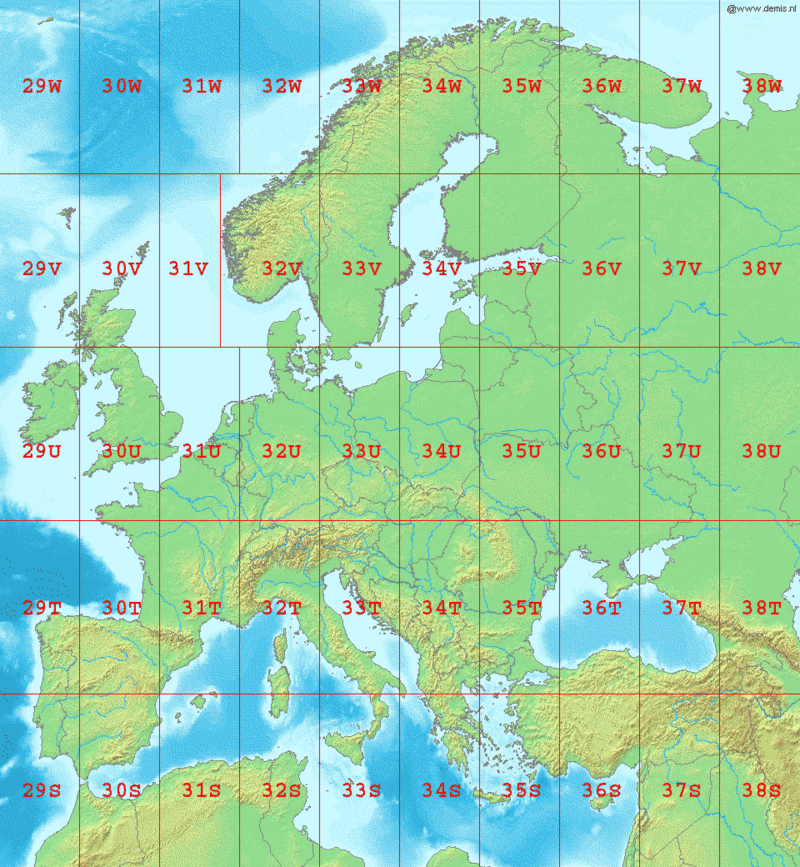
\includegraphics[scale=0.2]{secteurUTM.png} 
\captionof{figure}{Secteur UTM}
\label{fig1}
\end{center}

This figure show that we are currently in the sector 30. Whereas,in order to compute UTM coordinates, we need first to choose a geodesic system representing the Earth. For this project we chose the WGS-84 system which is the most commonly used system.


\end{document}
\section{Structure of the programming code}


Quatre scripts python: GPS2.py, commande.py, testserial.py et ServeurN.py

The code which have been implemented for this part of the project can be sum up with the following picture \ref{fig:SyntheseCodeRegulationRobot}:

\begin{figure}[ht]
\centering
    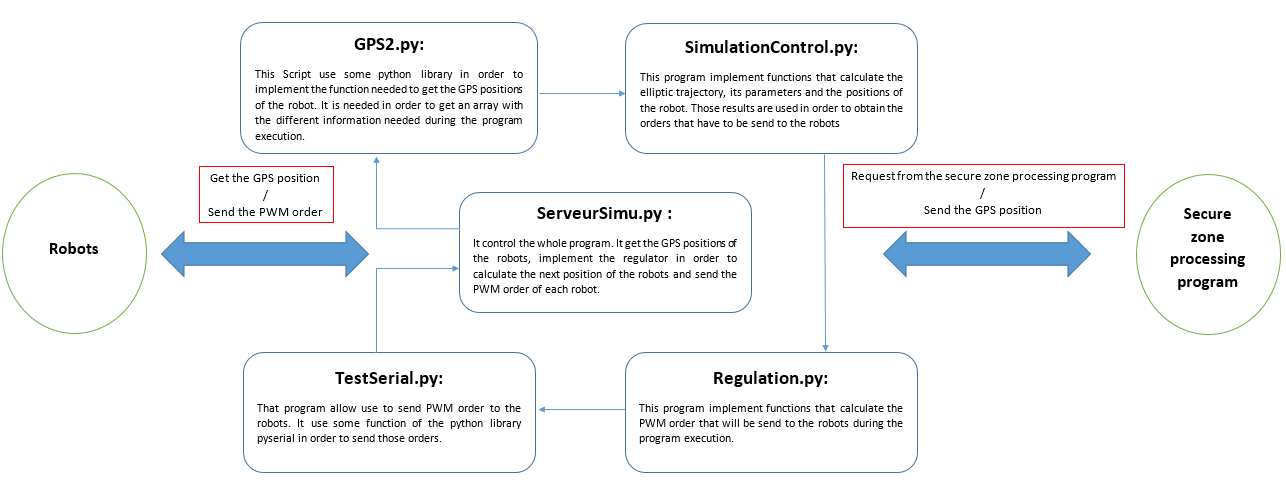
\includegraphics[scale=0.5,angle=90]{SyntheseCodeRegulationRobot.PNG}
    \caption{Architecture of the program which control the regulation of the robots.}
    \label{fig:SyntheseCodeRegulationRobot}
\end{figure}

As you can see, there are 5 main script that are used in order to run the whole program.

\begin{itemize}
\item \textbf{GPS2.py}: this script has been implemented by \textcolor{blue}{\textit{Pierre JACQUOT}} and allow us to get access to the GPS signal of all the robots. This programm catch the first available GPS tram og each robot, put it in a numpy array. The parameters which are keept are the latitude, the longitude, the speed, the north, the east and the time.
\item SimulationControl.py has been implemented by  \textcolor{blue}{\textit{Alice Danckaers}} and is used here in order to get the elliptic trajectory in function of the instant t and the theoretical position of each robots.

\end{itemize}
\pagebreak

\section{Results}
In the end, all the secure zone processing algorithm worked and gave excellent results. Nevertheless, due to some GPS tram issues, we couldn't succeed to do regulation during our demonstration.


\begin{center}
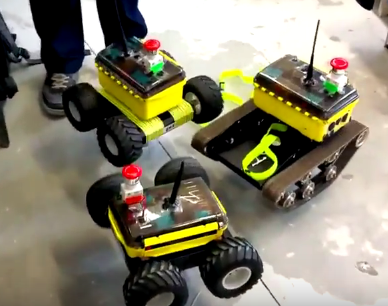
\includegraphics[scale=0.6]{Resultats2.png} 
\captionof{figure}{Robot implementation	}
\label{resultats2}
\end{center}

Nevertheless, we succeed to use robots in order to print the secure zone around them. The result is shown in the figure below.

\begin{center}
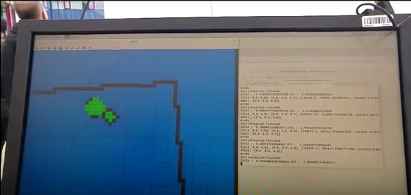
\includegraphics[scale=0.6]{Resultats1.png} 
\captionof{figure}{Results of our demonstration	}
\label{Resultats1}
\end{center}

%----------------------------------------------------------------------------------------
%	PART V 
%----------------------------------------------------------------------------------------
\chapter*{Conclusion}
\addcontentsline{toc}{chapter}{Conclusion}
\input{conclusion}

%----------------------------------------------------------------------------------------
\appendix
\chapter*{Appendix}
\addcontentsline{toc}{chapter}{Appendix}
\chapter{Appendix 1}
\chapter{Appendix 2}
\chapter{Appendix 3}

%----------------------------------------------------------------------------------------
%	BIBLIOGRAPHIE
%----------------------------------------------------------------------------------------
\addcontentsline{toc}{part}{Bibliography}
%\bibliographystyle{apalike-fr}
\bibliographystyle{plain-fr}
\bibliography{bibliographie}
\nocite{*}

%----------------------------------------------------------------------------------------

\end{document}